% LLNCStmpl.tex
% Template file to use for LLNCS papers prepared in LaTeX
%websites for more information: http://www.springer.com
%http://www.springer.com/lncs

\documentclass{llncs}
%Use this line instead if you want to use running heads (i.e. headers on each page):
%\documentclass[runningheads]{llncs}
\usepackage{url}
\usepackage[spanish]{babel}
\usepackage[utf8]{inputenc}
\usepackage{graphicx}
\usepackage{amsmath}
\usepackage{ntheorem}




\setlength{\theorempreskipamount}{7mm}
\setlength{\theorempostskipamount}{7mm}
\theoremstyle{plane}
\theorembodyfont{\normalfont}
\theoremheaderfont{\scshape\large}
\newtheorem{teo}{Teorema}
\newtheorem{defi}{Definición}
\newtheorem{ej}{Ejemplo}



\begin{document}
\title{Resumen  del documento: ''A Statistical Test Suite for Random and Pseudorandom Number Generators for Cryptographic Applications''}



\subtitle{Conceptos y aplicaciones.}

%For a single author
%\author{Author Name}

%For multiple authors:
\author{Marcos Daniel Calderón Calderón}


\institute{Centro de Investigación en Matemáticas \\ \email{marcos.calderon@cimat.mx}}



\maketitle

\begin{abstract}
En este documento se destacan algunos aspectos acerca de la selección y prueba de generadores de números aleatorios y peudoaleatorios. Las salidad de los generadores pueden ser utilizadoas en muchas aplicaciones criptográficas, así como para la generación de claves. En particular, las salidad deben ser impredecibles cuando no se tiene conocimiento sobre las entradas para la función generadora. El propósito de pruebas estadísticas y su relación con  el campo del criptoanálisis también es discutida, también se mencionan algunas pruebas estadísiticas. Dichas pruebas deben determinar si es adecuada una aplicación criptográfica analizada.  
\end{abstract}
\section{Introducción a las pruebas en números aleatorios.}

La necesidad de aleatoriedad y pseudoaleatoriedad de números es necesaria en muchas aplicaciones criptográficas. Por ejemplo, los criptosistemas utilizan claves que deben ser generadas en un ambiente aleatorio. Muchos protocolos criptográficos también requieren entradas aleatorias o pseudoaleatorias.
En este documento, se describen algunas pruebas estadísiticas para determinar aleatoriedad. Dichas pruebas están aprobadas por el Instituto Nacional de Estándares y Tecnología (NIST): las pruebas que se describen son capaces de detectar desviaciones en la aleatoriedad de una secuencia binaria.  

\subsection{Generalidades.}
Hay dos tipos básicos de generadores para producir secuencias aleatorias: \textbf{generadores de números aleatorios} (RNGs) y\textbf{ generadores de números pseudoaleatorios} (PRNGs). Para aplicaciones criptográficas, los dos tipos de generadores producen un flujo de ceros y unos que pueden ser divididos en pequeños fragmentos de números aleatorios.

\subsubsection{Aleatoriedad.}
Una secuencia aleatoria de bits se interpreta como el resultado de lanzar una moneda donde sus lados están etiquetados con los símbolos ''0'' y ''1'', donde cada una de estas etiquetas tiene la probabilidad de $\frac{1}{2}$ de que al caer la moneda se obtenga uno de los dos símbolos. El resultado de lanzamientos anteriores, no afecta futuros lanzamientos, esto significa que los lanzamientos son independientes. Una moneda con las características descritas es un generador perfecto de flujos aleatorios de bits, por lo tanto el ''0'' y el ''1'' están uniformemente distribuídos. Todos los elementos de la secuencia son generados de manera independiente, y el valor del siguiente elemento de la secuencia no puede ser predicho, a pesar de cuántos elementos se hayan producido.  

Como el uso de monedas justas para propósitos criptográficos es impráctico. Sin embargo, la salida hipotética de este generador idealizado sirve como un punto de referencia para la evaluación de los generadores de números aleatorios que se han propuesto con el tiempo.


\subsubsection{Imprevisibilidad}
Números aleatorios y pseudoaleatorios generados para aplicaciones criptográficas deben ser impredecibles. En el caso de los PRNGs, si la semilla es desconocida, la siguiente salida en la secuencia debe ser impredecible a pesar de tener conocimiento de números aleatorios previos generados en la secuencia. Esta propiedad es conocida como imprevisibilidad hacia adelante. De la misma manera, no debe ser posible determinar la semilla de cualquiera de los valores generados, es decir, también se requiere imprevisibilidad hacia atrás. No debe existir una correlación entre la semilla y cualquier valor generado a partir de una semilla. 

Asimismo, no debe ser posible determinar la semilla del conocimiento
de cualquiera de los valores generados (es decir, también se requiere imprevisibilidad hacia atrás). No existe correlación entre una semilla y el siguiente valor generado.

Para asegurar imprevisibilidad, se debe tener cuidado en las semillas que se obtienen. Los valores producidos por un PRNG son completamente previsibles si la semilla y el algoritmo de generación son conocidos. Como en muchos casos, el algoritmo de generación es públicamente conocido, la semilla se debe de mantener secreta y no debería ser descubierta de la secuencia de números pseudoaleatorios que esta produce. En conclusión la semila debe ser imprevisible.


\subsubsection{Generadores de Números Aleatorios.}
EL primer tipo de generador de secuencias de bits es el RNG. Este tipo de generadores utilizan una fuente no determinística, como la entropía y alguna función de procesamiento para producir aleatoriedad.

El uso de un proceso de destilación es necesario para superar cualquier debilidad en la fuente de entropía y que pudiera provocar que se generen valores no aleatorios. La fuente de entropía normalmente consiste en alguna cantidad física, como el ruido de un circuito eléctrico o los efectos cuánticos de un semiconductor.

\subsubsection{Generadores de Números Pseudoaleatorios.}
Un PRNG utiliza una o más entradas y genera múltiples números pseudoaleatorios. Las entradas a los PRNGs son semillas. En contextos en los cuales la imprevisibilidad es necesaria, la semilla por sí misma debe ser aleatoria e imprevisible. Por lo tanto, por defecto, un PRNG debería obtener sus semillas de la salida de RNG, esto significa que un PRNG necesita un RNG para trabajar juntos.

La salida de un PRNG es una función deterministica por parte de la semilla, esto significa que la aleatoriedad es debida a la elección de la semilla. La naturaleza determinística del proceso origina el concepto ''pseudoaleatorio''. Como cada elemento de una secuencia pseudoaleatoria es reproducible dada una semilla específica, únicamente la semilla necesita ser guardada si la reproducción o validación de la secuencia pseudoaleatoria es requerida. 

Irónicamente, los números pseudoaleatorios son más aleatorios que los números aleatorios obtenidos de fuentes físicas. Si una secuencia pseudoaleatoria es construída de manera apropiada, cada valor en la secuencia es producido de los valores previos con una transformación  que dr utiliza para introducir aleatoriedad artificial. Por lo tanto, la salida de un PRNG puede tener mejores propiedades estadísticas que un algoritmo RNG. Además de que la salida de un PRNG puede calcularse de una manera mas rápida.


\subsubsection{Pruebas.}

Varias pruebas estadísticas pueden ser aplicadas a una secuencia de bits aleatorios para compararla y evaluarla con una secuencia que es realmente aleatoria. Aleatoriedad es una propiedad probabilística; esto significa que las propiedades de una secuencia pueden ser caracterizados y descritos en términos de probabilidad. 
El resultado más probable de pruebas estadísticas, cuando se aplica a secuencias aleatorias reales, es conocido a priori y puede ser descrito  en términos probabilísticos. Hay un número infinito de pruebas estadísticas posibles, cada una es capaz de detectar la ausenca o presencia de patrones en la secuencia: si hay patrones detectados, la secuencia no es aleatoria.


Una prueba estadística es formulada para probar una hipótesis nula $H_{0}$. En el tema que estamos tratando en este documento, la hipótesis nula que se pondrá a prueba es que la secuencia es aleatoria. También se tiene una hipótesis alternativa $H_{a}$, ésta nos dice que la la secuencia a prueba no es aleatoria. EN cada prueba aplicada, se obtiene una decisión que acepta o rechaza la hipótesis nula $H_{0}$, es decir, si el generador produce o no valores aleatorios. 

Para cada test, un estadístico de aleatoriedad debe ser elegido y utilizado para determinar la aceptación o rechazo de la hipótesis nula. Bajo una suposición de aleatoriedad, tales estadísticos tienen una distribución de valores posibles. Una distribución teórica de referencia de sus estadísticos bajo la hipótesis nula es determinada por métodos mastemáticos. De esta distribución de referenci, un \textbf{valor crítico} es determinado. Durante la prueba, un valor de la prueba estadística es calculado sobre los datos (la secuencia que está siendo probada). El valor de este test estadístico es comparado con el valor crítico. Si el valor de test estadísitco excede el valor crítico, la hipótesis nula es rechazada. De otro modo, la hipótesis nula es aceptada.
La prueba de hipótesis estadísticas tiene dos conclusiones posibles: aceptar $H_{0}$ o aceptar $H_{a}$. Si los datos son en realidad aleatorios, entonces, existe una probabilidad de rechazar $H_{0}$, esto es conocido como el error tipo I. Si los datos no son aleatorios y aún así, aceptamos aceptando la hipótesis nula, estamos cayendo en un error tipo II.
La probabilidad de caer en un error tipo I, con frecuencia es llamada el \textbf{nivel del significancia del text}. Esta probabilidad puede darse a priori, normalmente se representa por $\alpha$. Para la prueba $\alpha$ es la probabilidad de que la prueba indicará que la secuencia no es aleatoria cuando en realidad si lo es. Un valor común para $\alpha$ en criptografía es de alrededor de $0.01$.

La probabilidad de un error de tipo II, es denotada por $\beta$. Para la prueba $\beta$ es la probabilidad de que la prueba indique que la secuencia es aleatoria cuando en realidad no lo es. Un mal generador produce una secuenca que parece tener propiedades aleatorias.  A diiferencia de $\alpha$, $\beta$ no es un falor fijado. $\beta$ puede tomar muchos valores diferentes porque hay un infinito número de maneras que un flujo de datos puede ser no aleatorio. El cálculo de error tipo II es más dificil que el cálculo del error tipo I.

Uno de los principales objetivos de las pruebas de aleatoriedad es minimizar la probabilidad de cometer un error de tipo II, lo que se busca es minimizar la probabilidad de aceptar una secuencia como aleatoria y su generador como bueno cuando en realidad es todo lo contrario. Las probabilidades $\alpha$ y $\beta$ están relacionadas una con otra de acuerdo al tamaño $n$ de la secuencia probada de tal manera que si dos des estos parámetros pueden ser especificados,  el tercer parámetro es automáticamente determinado.



\section{Pruebas para la generación de números aleatorios.}
Las pruebas que se mencionan en este documento son las siguientes:
\begin{enumerate}
\item The Frecuency (Monobit) Test.
\item Frecuency Test within a Block.
\item The Runs Test.
\item Tests for de Longest-Tun-of-Ones in a BLock.
\item The BInary Matrix Rank Test.
\item The Discrete Fourier Transform (Spectral) Test.
\item The Non-Overlapping Template Matching Test.
\item The Overlapping Template Matching Text.
\item Maurer's "Universal Statistical" Test,
\item The Linear Complexity Test,
\item The Serial Test,
\item The Approximate Entropy Test,
\item The Cumulative Sums (Cusums) Test,
\item The Random Excursions Test, and
\item The Random Excursions Variant Test.

\end{enumerate}

\subsection{Test de Frecuencia.}
El test de Frecuencia mide la proporción de ceros y unos de la secuencia entera. EL propósito del test es determinar si el número de ceros y unos en una secuencia es aproximadamente el mismo  como se debería esperar para una secuencia verdaderamente aleatoria.

La prueba evalúa la cercanía de la fracción  a $\frac{1}{2}$. Esto sisgnivida que el número de ceros u unos en una secuencia debería ser el mismo. 

\subsubsection{Regla de decisión con un nivel de 0.1}
Si el $P-valor$ obtenido es $<0.01$, se puede concluir que la secuencia no es aleatoria. De otro modo, concluimos que la secuencia es aleatoria.
\subsubsection{Conclusión e interpretación de los resultados.}
COmo el $P-valor$ obtenido es $\geq 0.01$, recordemomos que $P-valor =0.527089$, la conclusion es que la secuencia es aleatoria.
\subsubsection{Recomendación del tamaño de la entrada.}
Se recomienda que el tamaño de cada secuencia de entrada sea de mínimo 100 bits.


\subsection{Test de Frecuencia en Bloque.}
El test se concentra en medir la proporción de unos en bloques de M bits. EL propósito de el text es determinar si la frecuencia de unos en un bloque de tamaño $M$ es de aproximadamente $\frac{M}{2}$, como se debería esperar si se sigue la suposición de aleatoriadad en los bloques. Si el tamaño de los bloques fuera de uno $M=1$, este dest se coviernte en el test de Frecuencia.

\subsubsection{Regla de decisión con un nivel de 0.1}
Si el $P-valor$ obtenido es $<0.01$, se puede concluir que la secuencia no es aleatoria. De otro modo, concluimos que la secuencia es aleatoria.
\subsubsection{Conclusión e interpretación de los resultados.}
COmo el $P-valor$ obtenido es $\geq 0.01$, en el ejemplo de esta prueba $P-valor =0.801252$, la conclusion es que la secuencia es aleatoria.
Debemos de notar que si los $P-valor$ son muy pequeños, esto debería indicar una desviación muy grande de una proporción de ceros y unos en al menos  uno de los bloques.

\subsubsection{Recomendación del tamaño de la entrada.}
Se recomienda que cada secuencia a probar tenta un tamaño de mínimo 100 bits. El tamaño del bloque M debería ser elegido de tal manera que $M \geq 20$.

\subsection{The Runs Test.}
El propósito de este test es el número total de corridas en la secuencia, donde una corrida es una secuenci ininterrumpida de bits idénticos. Una corrida de tamaño \textit{k} consiste de \textit{k} bits idénticos y están rodeados antes y después por bits de valor opuesto. El propósito de este test es determinar si el número de corridas de ceros y unos de variso tamaños es el esperado para una secuencia aleatoria. EN particular esta prueba determina si la oscilación entre ceros y unos es rápida o lenta.
\subsubsection{Regla de decisión con un nivel de 0.1}
Si el $P-valor$ obtenido es $<0.01$, se puede concluir que la secuencia no es aleatoria. De otro modo, concluimos que la secuencia es aleatoria.
\subsubsection{Conclusión e interpretación de los resultados.}
COmo el $P-valor$ obtenido es $\geq 0.01$, en el ejemplo de esta prueba $P-valor =0.147232$, la conclusion es que la secuencia es aleatoria.
Debemos de fijarnos que un valor grande de $V_{n}(obs)$ debería de indicar una oscilación en la cadena que es muy rápida; un valor pequeño debería indicar que la oscilación es pequeña. (Una oscilación es un cambio de un cero a un uno y viceversa.) Una oscilación rápida ocurre cuenao hay muchos cmabios. Un flujo con basa oscilación tiene menos corridas que las que una secuencia aleatoria debería tener. Por ejemplo, una secuencia que contiene 100 unos, seguida de 73 ceros, seguida por 127 unos, para dar un total de 300 bits, tiene únicamente tres corridad, sin embargo, se esperan 150 corridas.

\subsubsection{Recomendación del tamaño de la entrada.}
Se recomienda que cada secuencia a probar tenta un tamaño de mínimo 100 bits. 


\subsection{Tests for de Longest-Tun-of-Ones in a BLock.}
\subsection{The Binary Matrix Rank Test.}
\subsection{The Discrete Fourier Transform (Spectral) Test.}
En este test lo que se hace es encontrar las alturas pico de la Transformada Discreta de Fourier de la secuencia. El propósito de este test es detectar patrones repetitivos que están cerca entre sí.  Estos patrones deben indicar que hay una desviación de la hipótesis de aleatoriedad. La intención es detectar si el número de picos exceden el $95\%$ de ubmral.


\subsection{The Non-Overlapping Template Matching Test.}
EL propósito de este test es el número de ocurrencias de cadenas pre especifidades. Se busca detectar generadores que produzcan muchas ocurrencias de un patrón aperiódico. Se utiliza una ventana de tamaño $m$ para buscar patrones. Si el patrón no se encuentra, entonces la ventana se recorre un bit. Si el patrón es encontrado, entonces la ventada es reinciada con el patrón de la nueva posición y se reanuda la búsqueda.


\subsection{The Overlapping Template Matching Text.}
El propósito de este test es el número de ocurrencias de una cadena específica de tamaño $m$, sin embargo, la diferencia con el método anterior es que cuando un patrón es encontrado, la ventana se despala sólo un bit antes de reiniciar la búsqueda.



\subsection{Maurer's ''Universal Statistical'' Test.}
The focus of this test is the number of bits between matching patterns (a measure that is related to the
length of a compressed sequence). The purpose of the test is to detect whether or not the sequence can be
significantly compressed without loss of information. A significantly compressible sequence is
considered to be non-random.

EL test descrito en esta parte se centra en el número de bits entre patrones reconocidos, (una medida que es relacionada con la longituda de una secuencia comprimida). El propósito del text es detectar si la secuencia se puede comprimir de manera significativa sin pérdida de información. Una secuencia que se pueda comprimir de manera significante, es considerada como no aleatoria.

\subsection{The Linear Complexity Test.}
Éste test utiliza la longitud de el linear feedback shift register (LFSR). EL propósito de este test es determinar si la secuencia es suficientemente compleja para ser considerada aleatoria. Secuencias aleatorias tienen LFSR más grandes. Una LFSR que es muy pequeña, implica que la secuencia no es aleatoria.

\subsection{The Serial Test.}


\subsection{The Approximate Entropy Test.}
\subsection{The Cumulative Sums (Cusums) Test.}
\subsection{The Random Excursions Test.}
\subsection{The Random Excursions Variant Test.}


\section{Descripción Técnica de las pruebas.}
\section{Estrategias de prueba y resultados de la interpretación.}

\subsection{Estrategias para el análisis estadístico de un RNG.}
En la práctica hay muchas estrategias distintas empleadas en el análisis estadístico de generadores de números aleatorios. NIST ha adoptado una arquitectura de 5 pasos involucrados en las pruebas estadísticas de generación de números aleatorios.

\subsubsection{Etapa 1. Selección de un generador.}
En esta etapa, se selacciona un generador basado en software y hardware para evaluar. El generador debe producit una secuencia binaria de ceros y unos de una longitud $m$. 


\subsubsection{Etapa 2. Generador de secuencias binarias.}
Para un tamaño fijo de secuencia $n$ y el generador elegido, construímos un conjunto de $m$ secuencias binarias y guardamos las secuencias en un archivo.

\subsubsection{Etapa 3. Ejecución del conjunto de pruebas estadísticas.}
En este paso, llamamos conjunto de pruebas estadísticas utilizando el archivo creado en la etapa 2 y el tamaño deseado de las secuencias. Seleccionamos los tests estadísticos y se asignan los parámetros de entrada de acuerdo a la prueba. 

\subsubsection{Etapa 4. Examen de los $P-valores$.}
Un archivo de salida será generado por el test, dicho archivo contiene valores intermedios importantes, como estadísticos de prueba y $P-valores$ para cada estadístico de prueba. Basado en estos $P-valores$, una conclusión con respecto a dichos valores puede haberse obtenido.

\subsubsection{Etapa 5. Evaluación aceptado o no aceptado.}
Para cata test estadístico, un conjunto de $P-valores$ es producido. Para un nivelo de significacncia fijo, un cierto porcentaje de $P-valores$ pueden indicar que la secuencia no es aleatoria. Por ejemplo, si al nivel de significancia se le asigna el valor de $0.01$, entonces se espere que un $1\%$ de las secuencias no sean aleatorias. Una secuencia aprueba el text estadístico siempre que $P-value \geq \alpha$. Para cada test estadístico, la proporción de secuencias que pasan es calculado y analizado. 


\subsection{La interpretación de resultados empíricos.}

Tres escenarios pueden ocurrid debido a las pruebas empíricas. Caso 1: El análisis del $P-valor$ no indican una desviación de la aleatoriedad. Caso 2: El análisis indica claramente una desviación de la aleatoriereda. Caso 3: No se pueden obtener conclusiones del análisis.

La interpretación de resultados empíricos puede ser 


\section{Guía de Usuario.}
Esta sección describe el proceso de intalación de las pruebas estadísticas desarrolladas por NIST.

\subsection{Descripción del paquete.}
El código que conforma las pruebas estadísticas fué diseñado específicamente para realizar pruebas estadísiticas a los PRNGs y RNGs. Varias implementaciones de los PRNGs utilizados durante la fase de desarrollo de el proyecto también han sido incluídos.

El paquete será útil en los siguientes casos:
\begin{itemize}
\item INdentificar si los PRNGs o RNGs a prueba producen secuencias binarias donde es posible identificar un patrón.
\item Para el diseño de nuevos (P)RNGs.
\item Verificacion de que que la implementación de un nuevo (P)RNG es la correcta. 
\item Revisión de los (P)RNGs estándar. 
\item Investigar el grado de aleatoriedad de el (P)RNG utilizado.
\end{itemize}

The objectives during the development of the NIST statistical test suite included:

\begin{itemize}

\item	 Platform Independence: The source code was written in ANSI C. However, some modification
may have to be made, depending on the target platform and the compiler.
\item		 Flexibility: The user may freely introduce their own math software routines.
\item		 Extensibility: New statistical tests can easily be incorporated.
\item		 Versatility: The test suite is useful in performing tests for PRNGs, RNGs and cipher algorithms.
\item	 Portability: With minor modifications, source code may be ported to different platforms. The
NIST source code was ported to a Windows XP system running Visual Studio 2005 compiler and
a Ubuntu Linux system running gcc.
\item	 Orthogonality: A diverse set of tests is provided.
\item	 Efficiency: Linear time or space algorithms were utilized whenever possible.
\end{itemize}

\subsection{Pasos para la intalación.}
\begin{itemize}
\item Copiamos el archivo \textbf{sts-2.1} al directorio de root y lo descomprimimos. Una instruccion válida para este paso es la siguiente: \textbf{sudo cp -r sts-2.1  /}.

\item Seis subdirectorios y un archivo se han de encontrar en la carpeta que ha sido creada. Los subdirectorios son:
\textbf{data/}, \textbf{experiments/}, \textbf{include/}, \textbf{obj/}, \textbf{src/} and \textbf{templates/}, el archivo es \textit{makefile}.



\item The experiments/ subdirectory will be the repository of the empirical results for the
statistical tests. Several subdirectories should be contained in it. These include
AlgorithmTesting/, BBS/, CCG/, G-SHA1/, LCG/, MODEXP/, MS/, QCG1/,
QCG2/, and XOR/. All but the first of these subdirectories is meant to store the
results for the corresponding PRNG. The AlgorithmTesting/ subdirectory is the
default subdirectory for empirical results corresponding to RNG data stored in the
data/ subdirectory.
\item 	 El  subdirectorio \textbf{include/} contiene los archivos de cabecera para las pruebas estadísticas, generadores de números aleatorios y rutinas asociadas.

\item 	 El subdirectorio \textbf{obj/} contienen los archivos del objeto correspondientes a las pruebas estadísticas, generadores de números pseudoaleatorios y otras rutinas asociadas.

\item EL subdirectorio \textbf{src/} contiene el código fuente para cada una de las pruebas estadísticas.

\item 	El subdirectorio \textbf{templates/} contiene un conjunto de plantillas para variar el tamaño de los bloques que serán utilizados en la prueba estadística: NonOverlapping Templates.

\item Las modificaciones hechas por el ususario pueden ser introducidad en varios archivos.


\end{itemize}

\section{Ejemplo para cada prueba.}
\subsection{Ejemplo sencillo.}

\begin{itemize}
\item Una cosa interesante en este programa, es que podemos agregar nuestros propios métodos para probar la aleatoriedad de una secuencia de bits, también podemos agregar nuestro propio generador de números pseudoaleatorios. 

\item Primero entramos a la carpeta que hemos descargado y ejecutamos el ejecutable assess. Se nos pide la siguiente información: seleccionar el tipo de generador de números pseudoaleatorios y elegir una prueba estadística para las secuencias generadas. Como se muestra en la figura ~\ref{ev} .

\begin{figure}[h!]
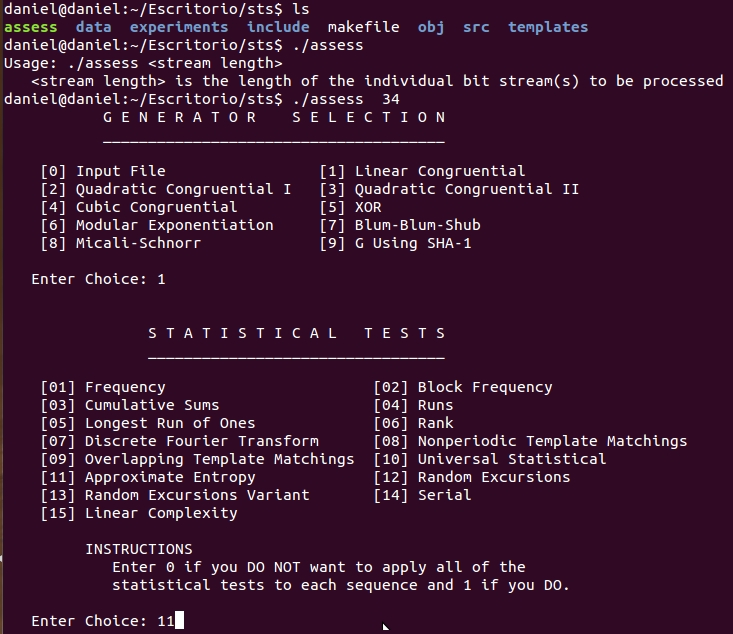
\includegraphics[width=10cm]{prueba1.jpg}
\caption{Información que nos pide el programa.}
\label{ev}
\end{figure}

\item Cuando elegimos el método que se va a utilizar para la evaluación de la aleatoriedad, se piden los parámetros específicos de cada método. 

\item Cuando el algoritmo termina de ejecutarse, se muestra la siguiente pantalla indicando que la operación se ha realizado con éxito:
~\ref{ev2} .

\begin{figure}[h!]
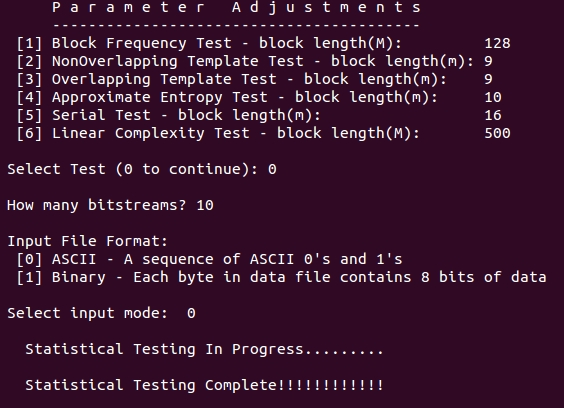
\includegraphics[width=10cm]{prueba2.jpg}
\caption{Salida con éxito del programa.}
\label{ev2}
\end{figure}

\item A la hora de hacer la ejecución, podemos elegir la opción de ejecutar sólo un algoritmo para  el análisis de los datos, o si se ejecutan todos los algoritmos para el mismo archivo, dependiendo de la elección, el análisis nos devolverá dos archivos: uno con el nombre \textbf{results.txt} y otro con el nombre \textbf{stats.txt}. Por ejemplo, en la carpeta que guarda los resultados del método de \textbf{CUMULATIVE SUMS (FORWARD)} se obtuvo el siguiente resultado:

\begin{verbatim}
  CUMULATIVE SUMS (FORWARD) TEST
		-------------------------------------------
		COMPUTATIONAL INFORMATION:
		-------------------------------------------
		(a) The maximum partial sum = 16
		-------------------------------------------
SUCCESS		p_value = 0.219194

		      CUMULATIVE SUMS (REVERSE) TEST
		-------------------------------------------
		COMPUTATIONAL INFORMATION:
		-------------------------------------------
		(a) The maximum partial sum = 19
		-------------------------------------------
SUCCESS		p_value = 0.114866

		      CUMULATIVE SUMS (FORWARD) TEST
		-------------------------------------------
		COMPUTATIONAL INFORMATION:
		-------------------------------------------
		(a) The maximum partial sum = 24
		-------------------------------------------
SUCCESS		p_value = 0.032790

		      CUMULATIVE SUMS (REVERSE) TEST
		-------------------------------------------
		COMPUTATIONAL INFORMATION:
		-------------------------------------------
		(a) The maximum partial sum = 24
		-------------------------------------------
SUCCESS		p_value = 0.032790

		      CUMULATIVE SUMS (FORWARD) TEST
		-------------------------------------------
		COMPUTATIONAL INFORMATION:
		-------------------------------------------
		(a) The maximum partial sum = 11
		-------------------------------------------
SUCCESS		p_value = 0.540731

		      CUMULATIVE SUMS (REVERSE) TEST
		-------------------------------------------
		COMPUTATIONAL INFORMATION:
		-------------------------------------------
		(a) The maximum partial sum = 12
		---------------------------------------
\end{verbatim}

\end{itemize}


\subsection{Ejemplo para la prueba de frecuencias.}

Esta prueba lo que nos pide es un flujo de bits de una tamaño de minimo 100. 
Vamos a asignar los datos del archivo ''data.pi'', a la hora de ejecutar esta prueba, obtenemos el siguiente resultado:
\begin{verbatim}
		      FREQUENCY TEST
		---------------------------------------------
		COMPUTATIONAL INFORMATION:
		---------------------------------------------
		(a) The nth partial sum = -16
		(b) S_n/n               = -0.160000
		---------------------------------------------
SUCCESS		p_value = 0.109599
\end{verbatim}

Como se puede ver en los resultados, $P-valor>0.1$ y se puede concluir que el flujo de bits que se ha puesto a prueba es aleatorio.


\subsection{Ejemplo para la prueba de runs.}
En este ejemplo, se utiliza la prueba de runs, en este caso, la aleatoriedad se mide por la cantidad de veces que ocurre un cambio de 0 a 1 y viceversa. Si tenemos 100 bits, se espera que existan 50 cambios.

\begin{verbatim}
		------------------------------------------
		COMPUTATIONAL INFORMATION:
		------------------------------------------
		(a) Pi                        = 0.420000
		(b) V_n_obs (Total # of runs) = 52
		(c) V_n_obs - 2 n pi (1-pi)
		    -----------------------   = 0.476049
		      2 sqrt(2n) pi (1-pi)
		------------------------------------------
SUCCESS		p_value = 0.500798
\end{verbatim}

\subsection{Ejemplo para la prueba de la transformada de Fourier.}


\begin{verbatim}
				FFT TEST
		-------------------------------------------
		COMPUTATIONAL INFORMATION:
		-------------------------------------------
		(a) Percentile = 96.000000
		(b) N_l        = 48.000000
		(c) N_o        = 47.500000
		(d) d          = 0.458831
		-------------------------------------------
SUCCESS		p_value = 0.646355
\end{verbatim}





%The bibliography, dne here without a bib file
%This is the old BibTeX style for use with llncs.cls
\bibliographystyle{splncs}

%Alternative bibliography styles:
%the following does the same as above except with alphabetic sorting
%\bibliographystyle{splncs_srt}
%the following is the current LNCS BibTex with alphabetic sorting
%\bibliographystyle{splncs03}
%If you want to use a different BibTex style include [oribibl] in the document class line

\begin{thebibliography}{1}
%add each reference in here like this:
\bibitem[RE1]{reference1}
Andrew Rukhin, Juan Soto, James Nechvatal, Miles
Smid, Elaine Barker, Stefan Leigh, Mark Levenson, Mark
Vangel, David Banks,Alan Heckert, James Dray, San Vo:  A Statistical Test Suite for
Random and Pseudorandom
Number Generators for
Cryptographic Applications :
National Institute of Standards and Technology Special Publication 800-22 revision 1a
Natl. Inst. Stand. Technol. Spec. Publ. 800-22rev1a, 131 pages (April 2010):
\end{thebibliography}

\end{document}

